\documentclass[titlepage,12pt,a4paper]{article}
\usepackage[a4paper]{geometry}
\usepackage{amsmath}
\usepackage{amssymb}
\usepackage{enumitem}
\usepackage{commath}
\usepackage{mathtools}
\usepackage{graphicx}
\usepackage{dirtytalk}
\usepackage{csquotes}
\usepackage{hyperref}
\usepackage{tabto}
\usepackage{gensymb}
\usepackage{graphicx}

\usepackage{fancyhdr}
\setlength{\headheight}{15.2pt}
\pagestyle{fancy}
\fancyhf{}
\lhead{ \fancyplain{}{COMP3431: Robotic Software Architecture} }
\rfoot{ \fancyplain{}{\thepage} }


\begin{document}
\begin{titlepage}
    \begin{center}
        \vspace*{3cm}
        
        \Huge
        \textbf{COMP3431\\}
        \title{}
        \vspace{0.5cm}
        \Huge
        \textbf{Robotic Software Architecture}
        
        \vspace{0.54cm}
        
        \Large
        Assignment 1: Report
        
        \vspace{5cm}

	\normalsize
	Christopher Manouvrier\\
	Aaron Ramshaw\\
	Simon Robilliard\\
	Oliver Tan\\
	Aneita Yang
        
	\vfill
        
        \Large
        September 5, 2015
        
    \end{center}
\end{titlepage}

\pagebreak

\section*{Exploration}

FastSLAM - good enough resolution, we don't care about 0.01 HectorSLAM res

Before it can drive around the maze autonomously, the TurtleBot must first explore the maze to generate a map that can be used in later modules. \\
\\
A wall-follower, although guaranteed to map out the entire maze correctly, has limitations in its speed. It often spends more time than is necessary to finish mapping a location, following any walls it comes across, regardless of any existing knowledge about the area.\\
\\
To speed up the exploration of the unknown maze, a Dijkstra's search is performed on any existing data we have of the maze. This data is delivered to us in the form of an OccupancyGrid message, which publishes an array of integers representing knowledge of the maze.


\pagebreak


\section*{Beacon Recognition and Localisation}

During the TurtleBot's first exploration of the maze, the camera is used to identify and position beacons. For every image frame captured by the Bot, we generate four additional images (for pink, yellow, blue and green), which only display the regions that lie within their colour thresholds. OpenCV's SimpleBlobDetector is used to extract the colour "blobs" from our images.\\
\\
To minimise the number of false positives and to distinguish between beacons and background colour noise, the SimpleBlobDetector filters by area, inertia and convexity and looks for areas in an image which satisfy the following criteria:

	\begin{enumerate}
		\item Area of the coloured region in the image is at least 200 pixels.
		\item Inertia of the detected region is greater than 0.65.
		\item Detected blob has a minimum convexity of 0.5.\\
	\end{enumerate}

\noindent
OpenCV's drawKeypoints is used to retrieve the location, as pixel values, of each detected colour region within an image. We conclude that a beacon has been successfully detected if there are two "blobs" in the same image frame within a 20 pixel offset from each other in the horizontal axis. This threshold of 20 pixels is used to account for any motion blur. The beacon's top colour is determined by comparing the two keypoints' y values.\\
\\
Pinpointing the locations of detected beacons is essential in order for the TurtleBot to complete Waypoint Traversal. Each beacon's position is determined by first considering the TurtleBot's position and orientation in the maze (i.e. relative to the origin of the map), and looking at data from the DepthCloud. \\
\\
To determine the rotation of the beacon from the origin of the map, we consider the pixel in the image at which the beacon was detected, relative to the centre pixel of the image. It is known that the camera has a 55\degree field-of-view and, thus, we are able to use these pixel values to calculate the beacon's rotation from the origin. \\
\\
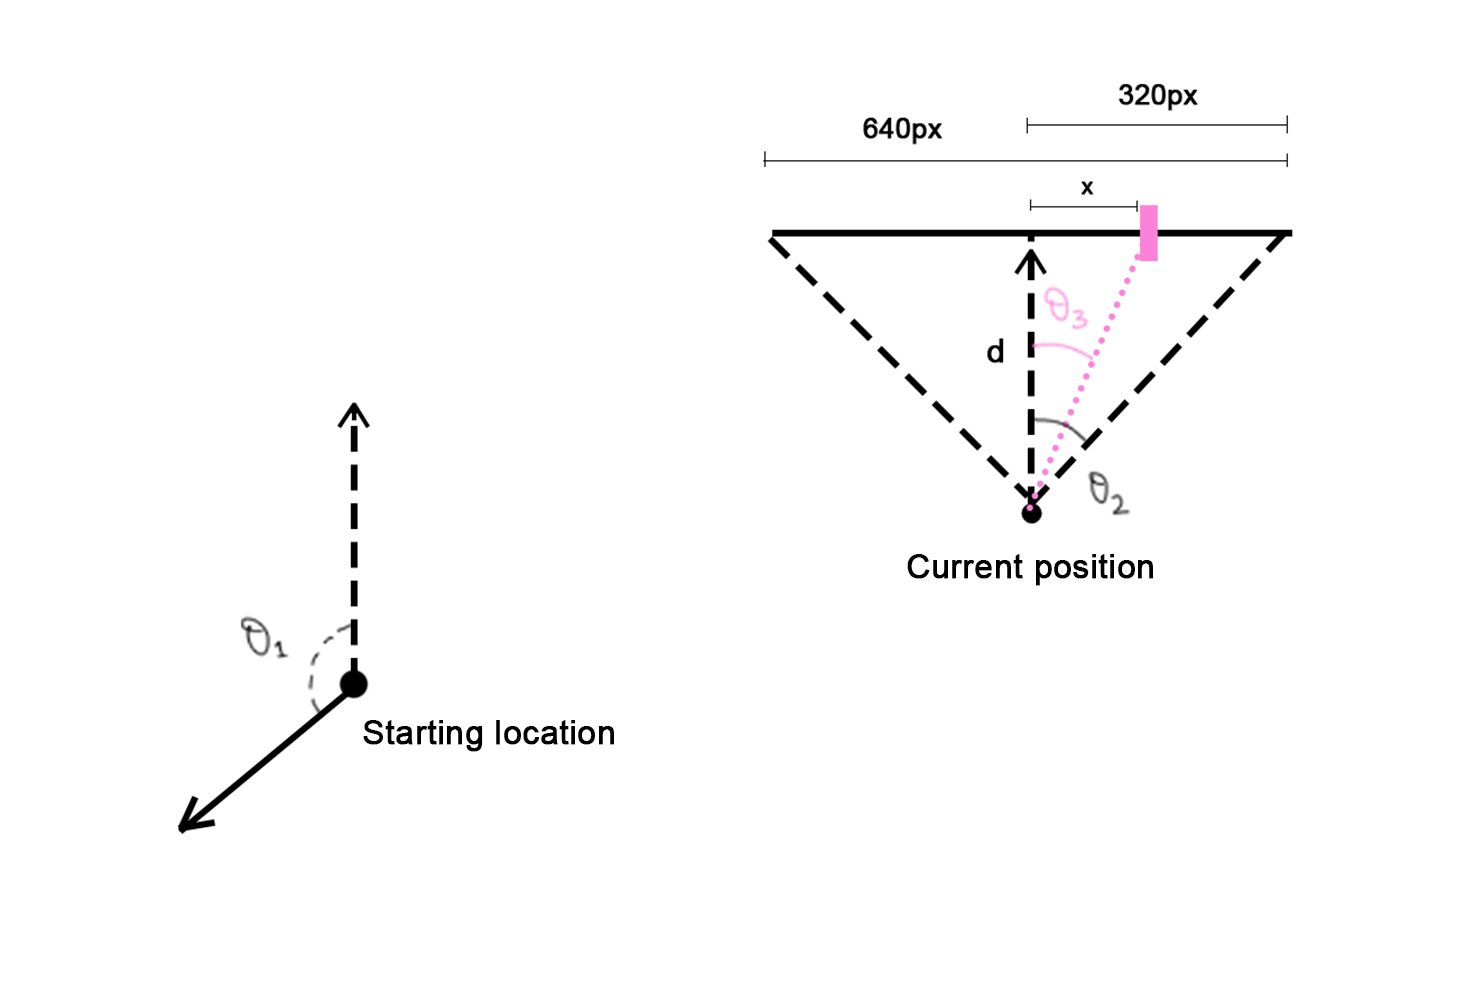
\includegraphics[scale=0.3]{beacon.jpg}

\begin{equation*}
	\theta_1   =  \mbox{TurtleBot's current yaw, relative to start} \\
\end{equation*}
\begin{equation*}
	\theta_2   =  27.5\degree \\
\end{equation*}

\begin{equation*}
	\begin{split}
		x = \mbox{vertical pixel in image at which beacon was detected} - 320\mbox{px}
	\end{split}
\end{equation*}

\begin{equation*}
	\begin{split}
		d &= \frac{320}{\tan{27.5\degree}}
	\end{split}
\end{equation*}

\begin{equation*}
	\begin{split}
		\theta_3 &= \tan^{-1}{(\frac{x}{d})}
	\end{split}
\end{equation*}

$\therefore$ the beacon's orientation from origin of the map is $\theta_1 + \theta_3$. \\
\\
To determine the beacon's x and y coordinates in the map, we use the DepthCloud generated from the laser scan. \\
\\
TODO:\\
Beacon recognition does 'Planner' module
	- given the colours to visit, will keep track of where they are
	- returns their positions in map coordinates (in order)
	- once all 4 beacons are found, we switch to waypoint traversal


\section*{Waypoint Traversal}

Once the maze has been successfully mapped and the positions of all beacons has been detected, the TurtleBot's next task is to visit the specified beacons in order. To speed up this process, an A* search is performed on the available data - namely, the OccupancyGrid with beacon locations written into it.\\
\\
The A* search returns the path (as cells) from the TurtleBot's current location to it's goal.

- Heuristic: Euclidean distance

\section*{Planner}



\end{document}